\documentclass{article}
\usepackage{tikz}
\usetikzlibrary{shapes.geometric, arrows}
\usepackage[landscape]{geometry}

\tikzstyle{startstop} = [rectangle, rounded corners, minimum width=3cm, minimum height=1cm,text centered, draw=black, fill=red!30, scale=1.3, font=\large]
\tikzstyle{process} = [rectangle, minimum width=3cm, minimum height=0.8cm, text centered, draw=black, fill=orange!30, scale=1.3,
font=\large]
% \tikzstyle{decision} = [diamond, minimum width=1cm, minimum height=0.34cm, text centered, draw=black, fill=green!30]
\tikzstyle{decision} = [ellipse, minimum width=2cm, minimum height=1cm, text centered, draw=black, fill=green!30, scale=1.3,
font=\large]
\tikzstyle{arrow} = [thick,->,>=stealth, font=\large]

\begin{document}
\begin{landscape}
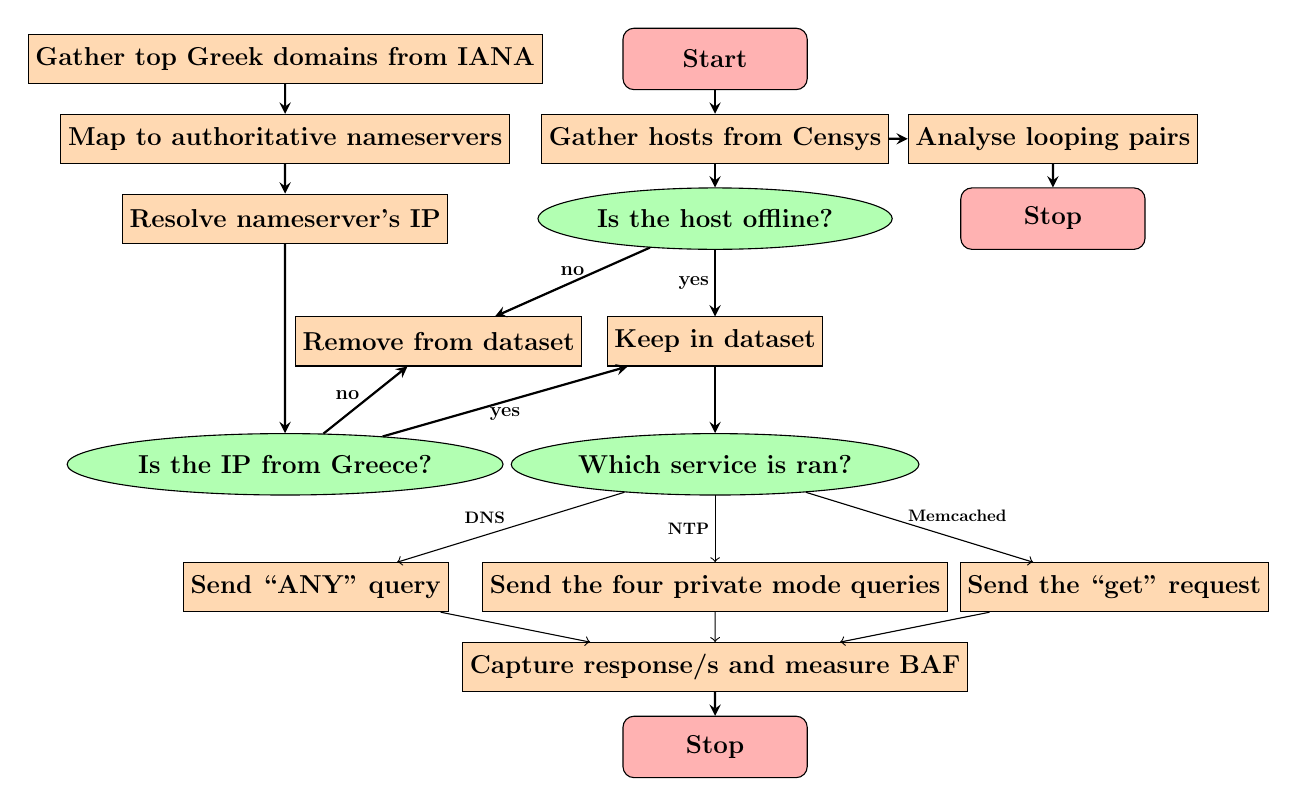
\begin{tikzpicture}[node distance=1cm, scale=0.6, transform shape]

% Nodes
\node (start) [startstop] {\textbf{Start}};
\node (gather) [process, below of=start, yshift=-0.3cm] {\textbf{Gather hosts from Censys}};
\node (check) [decision, below of=gather, yshift=-0.3cm] {\textbf{Is the host offline?}};
\node (remove) [process, left of=check, xshift=-3.5cm, yshift=-2cm] {\textbf{Remove from dataset}};
\node (keep) [process, below of=check, yshift=-1cm] {\textbf{Keep in dataset}};

% Authoritative name servers flow
\node (domains) [process, left of=start, xshift = -6cm] {\textbf{Gather top Greek domains from IANA}};
\node (nameservers) [process, below of=domains, yshift = -0.3cm] {\textbf{Map to authoritative nameservers}};
\node (ns_ips) [process, below of=nameservers, yshift = -0.3cm] {\textbf{Resolve nameserver's IP}};
\node (in_greece) [decision, below of=ns_ips, yshift=-3cm] {\textbf{Is the IP from Greece?}};



% Measure flow
\node (which_service) [decision, below of=keep, yshift = -1cm] {\textbf{Which service is ran?}};
\node (dns) [process, below of=which_service,   xshift=-6.5cm, yshift=-1cm] {\textbf{Send ``ANY'' query}};
\node (ntp) [process, below of=which_service, yshift = -1cm] {\textbf{Send the four private mode queries}};
\node (memcached) [process, below of=which_service, xshift=6.5cm, yshift=-1cm] {\textbf{Send the ``get'' request}};

\node (measure) [process, below of=ntp, yshift=-0.3cm] {\textbf{Capture response/s and measure BAF}};

\node (stop) [startstop, below of=measure, yshift=-0.3cm] {\textbf{Stop}};

\node (loopy) [process, right of=gather, xshift=4.5cm] {\textbf{Analyse looping pairs}};

\node (stop2) [startstop, below of=loopy, yshift=-0.3cm] {\textbf{Stop}};


% Arrows
\draw [arrow] (start) -- (gather);
\draw [arrow] (gather) -- (loopy);
\draw [arrow] (gather) -- node[anchor=east] {} (check);
\draw [arrow] (check) -- node[anchor=east] {\textbf{yes}} (keep);
\draw [arrow] (check) -- node[anchor=south] {\textbf{no}} (remove);

% Authoritative name servers flow
\draw [arrow] (domains) -- (nameservers);
\draw [arrow] (nameservers) -- (ns_ips);
\draw [arrow] (ns_ips) -- (in_greece);
\draw [arrow] (in_greece) -- node[anchor=north] {\textbf{yes}} (keep);
\draw [arrow] (in_greece) -- node[anchor=east, yshift=0.1cm] {\textbf{no}} (remove);
\draw [arrow] (keep) -- (which_service);

% Measure flow
\draw[->] (which_service) -- node[anchor=east, yshift=0.2cm] {\textbf{DNS}} (dns);
\draw[->] (which_service) -- node[anchor=east] {\textbf{NTP}} (ntp);
\draw[->] (which_service) -- node[anchor=south, xshift=0.8cm] {\textbf{Memcached}} (memcached);


\draw[->] (dns) -- (measure);
\draw[->] (ntp) -- (measure);
\draw[->] (memcached) -- (measure);

% \draw [arrow] (loopy) to[out=0, in=0, looseness=2.1] (stop2);
\draw [arrow] (loopy) -- (stop2);

\draw [arrow] (measure) -- (stop);


\end{tikzpicture}
\end{landscape}
\end{document}
